\documentclass[12pt]{article}
\usepackage[T1]{fontenc}
\usepackage[T1]{polski}
\usepackage[utf8]{inputenc}
\newcommand{\BibTeX}{{\sc Bib}\TeX} 
\usepackage{graphicx}
\usepackage{amsfonts}
\usepackage{multirow}

\setlength{\textheight}{21cm}

\title{{\bf Zadanie nr 1 - Klasyfikacja}\linebreak
Inteligentna analiza danych}
\author{Przemysław Zdrzalik, 224466 \and Karol Domański 224285}
\date{07 czerwca 2020 roku}

\begin{document}
\clearpage\maketitle
\thispagestyle{empty}
\newpage
\setcounter{page}{1}
\section{Cel zadania}

Celem zadania było wykorzystanie wielowarstwowego perceptronu (MLP) \\w celu klasyfikacji obiektów.

\section{Wstęp teoretyczny}

W zadaniu wykorzystujemy sieć neuronową o jednej warstwie ukrytej, jednym do czterech wejść oraz trzech wyjściach. \\Testujemy różne permutacje danych wejściowych. \\ Wszystkie warstwy posiadają sigmoidalne funkcje aktywacji. \\Sieć uczylismy metodą najszybszego spadku  korzystając z dwu różnych zbiorów treningowych, a naukę testowaliśmy na trzecim zbiorze testowym.\\
Jakość aproksymacji określaliśmy za pomocą błędu średniokwadratowego oraz poprzez procent poprawnie zaklasyfikowanych obiektów.\\ Obiekt uważamy za poprawnie zaklasyfikowany, jeżeli na odpowiadającym mu wyjściu sieć neuronowa wyprodukuje wartość największą, to znaczy wśród trzech wyjść sieci na wyjściu odpowiadającym obiektowi otrzymamy największą z trzech wartości.

\newpage
\section{Eksperymenty i wyniki} 

Wszystkie eksperymenty wykonujemy ustawiając numpy.random.seed() na wartość 0.

\subsection {Eksperyment 1}

Zaczynamy eksperymenty od testu wpływu ilości neuronów na jakość dopasowania.\\ W tym celu będziemy korzystać z sieci neuronowej z czterema,\\ czyli wszystkimi, wejściami. Rozpoczynamy od jednego neuronu.\\

\begin{figure}[!htb]
 \centering
 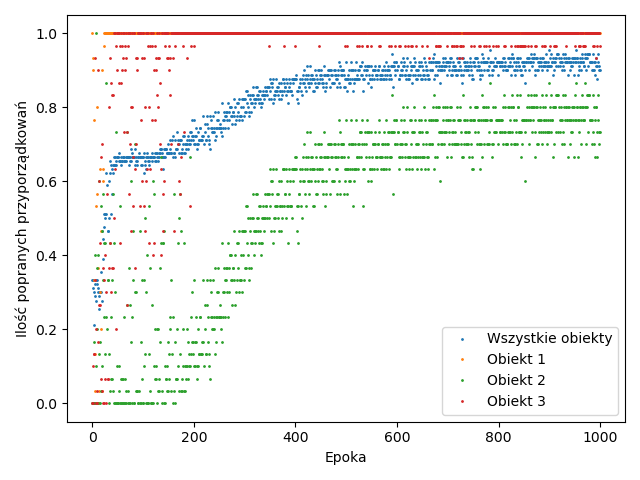
\includegraphics[width=12cm]{WykresPrzyporzadkowania1neuron4wejscia.png}
 \caption{Wykres Zmiany Jakości przyporządkowania dla 1000 epok}
 \vspace{-0.1cm}
 \label{WykresPrzyp1}
\end{figure}

Jak Widzimy z rysunku Rys. \ref{WykresPrzyp1}, 1 neruon poradził sobie z zadaniem klasyfikacji całkiem dobrze. Najlepiej, bo w 100\% poradził sobie z przyporządkowaniem klasy obiektowi nr. i 1. Gorzej bo w około 80\% przypadków Sieć poradziła sobie z przyporządkowaniem klasy 2.\\

\begin{table}
\caption{\label{tab:tablica1} Macierz Pomyłek dla 1 neuronu i 4 wejść }
\begin{tabular}{ |p{3cm}|p{3cm}|p{2cm}|p{2cm}|p{2cm}|  }
 \hline
 & & 
 \multicolumn{3}{|c|}{Przyporządkowane Klasy} \\
 \hline

   & & Klasa 1 & Klasa 2 & Klasa 3\\
 \hline
\multirow{3}{4em}{Klasy Źródłowe}
   & Klasa 1 & 31 & 0 & 0 \\ 
   & Klasa 2 & 2 & 25 & 4 \\
   & Klasa 3 & 0 & 0 & 31 \\

 \hline
\end{tabular}
\end{table}
\newpage

Widzimy tą zależność w \ref{tab:tablica1}  macierzy pomyłek, gdzie zauważamy że dla zbioru testowego Klasa 1 i 3 zostały przyporządkowane w 100\% przypadków w odróżnieniu od klasy 2.
\\Klasa 1 - Precision = 31 / 33, Recall = 31/31\\
Klasa 2 - Precision = 25/25 , Recall = 25/31\\
Klasa 3 - Precision = 31 / 35, Recall = 31 / 31\\


\begin{figure}[!htb]
 \centering
 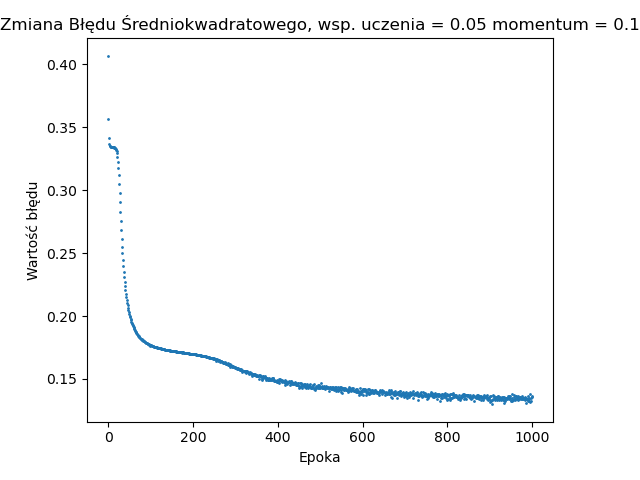
\includegraphics[width=12cm]{WykresBlad1neuron4wejscia.png}
 \caption{Wykres Zmiany Błędu Średniokwadratowego dla 1000 epok}
 \vspace{-0.1cm}
 \label{WykresBlad1}
\end{figure}

Jak mogliśmy się spodziewać błąd średniokwadratowy pozostaje wysoki ze względu na wpływ klasy 2.


\newpage

Powtarzamy eksperyment dla 3 neuronów w warstwie ukrytej.

\begin{figure}[!htb]
 \centering
 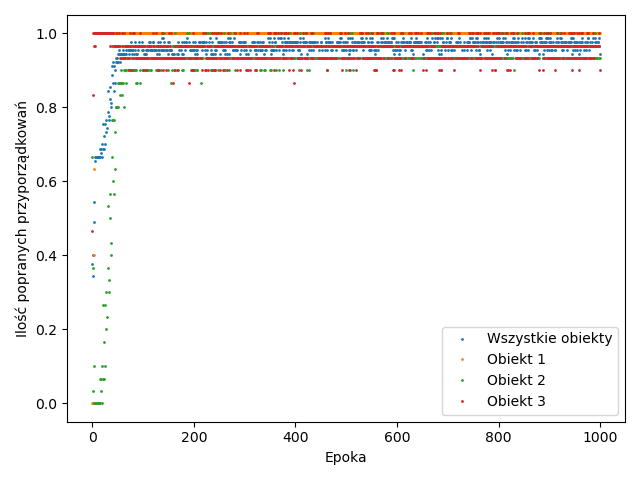
\includegraphics[width=11cm]{WykresPrzyporzadkowania3neuron4wejscia.png}
 \caption{Wykres Zmiany Jakości przyporządkowania dla 1000 epok}
 \vspace{-0.1cm}
 \label{WykresPrzyp2}
\end{figure}

\begin{figure}[!htb]
 \centering
 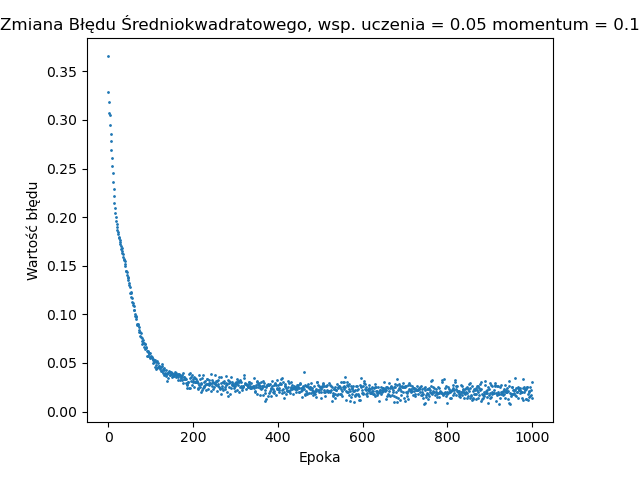
\includegraphics[width=11cm]{WykresBlad3neuron4wejscia.png}
 \caption{Wykres Zmiany Błędu Średniokwadratowego dla 1000 epok}
 \vspace{-0.1cm}
 \label{WykresBlad2}
\end{figure}

Od razu widzimy, że sieć poradziła sobie o wiele lepiej z klasyfikacją.\\


\begin{table}
\caption{\label{tab:tablica2} Macierz Pomyłek dla 3 neuronów i 4 wejść }
\begin{tabular}{ |p{3cm}|p{3cm}|p{2cm}|p{2cm}|p{2cm}|  }
 \hline
 & & 
 \multicolumn{3}{|c|}{Przyporządkowane Klasy} \\
 \hline

   & & Klasa 1 & Klasa 2 & Klasa 3\\
 \hline
\multirow{3}{4em}{Klasy Źródłowe}
   & Klasa 1 & 31 & 0 & 0 \\ 
   & Klasa 2 & 0 & 28 & 3 \\
   & Klasa 3 & 0 & 0 & 31 \\

 \hline
\end{tabular}
\end{table}

Zauważamy, że mimo diametralnej poprawy w przyporządkowaniu klasy 2 dla zbioru treningowego sieć przyporządkowała jedynie 3 obiekty poprawnie dla klasy 2 więcej w zbiorze testowym.
Dla tej próby Wszystkie obiekty klasy 1 zostały poprawnie rozpoznane, jednak błąd nadal pojawia sie przy rozróżnaniu klasy 3 i klasy 2.

Dalsze zwiększanie ilości neronów nie dawało zauważalnych różnic w klasyfikacji więc te pomiary pomijamy.
\\Klasa 1 - Precision = 31 / 31, Recall = 31/31\\
Klasa 2 - Precision = 28/28 , Recall = 28/31\\
Klasa 3 - Precision = 31 / 34, Recall = 31 / 31\\


\newpage

\subsection {Eksperyment 2}

Kontunuujemy eksperymenty na sieci neuronowej sprawdzając sieci z trzema wejściami.\\
Zaczynamy sprawdzając klasyfikację korzystając z pierwszych 3 parametrów.\\
Zaczynamy ponownie od sprawdzenia jakości dla jednego neuronu.\\ 

\newpage
\begin{figure}[!ht]
 \centering
 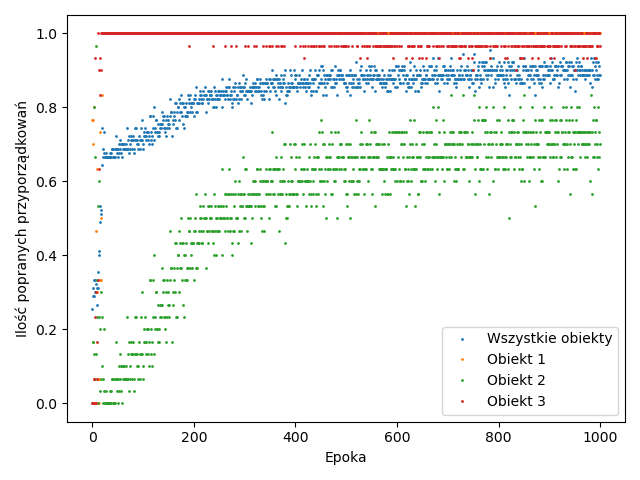
\includegraphics[width=11cm]{WykresPrzyporzadkowania1neuron3wejscia1.png}
 \caption{Wykres Zmiany Jakości przyporządkowania dla 1000 epok}
 \vspace{-0.1cm}
 \label{WykresPrzyp3}
\end{figure}

\begin{figure}[!ht]
 \centering
 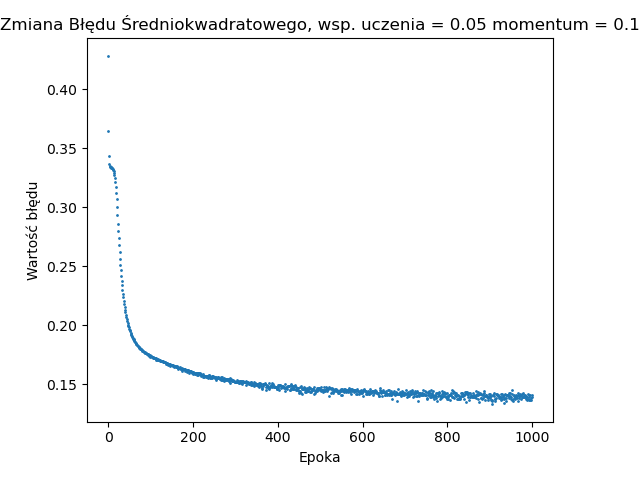
\includegraphics[width=11cm]{WykresBlad1neuron3wejscia1.png}
 \caption{Wykres Zmiany Błędu Średniokwadratowego dla 1000 epok}
 \vspace{-0.1cm}
 \label{WykresBlad3}
\end{figure}
\newpage

Nie zauważamy znacznych różnic w procesie nauki dla sieci.\\


\begin{table}
\caption{\label{tab:tablica3} Macierz Pomyłek dla 1 neuronu i 3 wejść }
\begin{tabular}{ |p{3cm}|p{3cm}|p{2cm}|p{2cm}|p{2cm}|  }
 \hline
 & & 
 \multicolumn{3}{|c|}{Przyporządkowane Klasy} \\
 \hline

   & & Klasa 1 & Klasa 2 & Klasa 3\\
 \hline
\multirow{3}{4em}{Klasy Źródłowe}
   & Klasa 1 & 31 & 0 & 0 \\ 
   & Klasa 2 & 2 & 27 & 2 \\
   & Klasa 3 & 0 & 3 & 28 \\

 \hline
\end{tabular}
\end{table}
Różnicę jednak widać w przyporządkowaniu dla zbioru testowego, \\ jak widać w macierzy pomyłek, tabela Tab. \ref{tab:tablica3} obserwujemy że przyporządkowanie dla klasy 3 nie jest już 100 procentowe.\\ Pomiary powtórzyliśmy dla 5 neuronów.
\\Klasa 1 - Precision = 31 / 33, Recall = 31/31\\
Klasa 2 - Precision = 27/30 , Recall = 27/31\\
Klasa 3 - Precision = 28/30, Recall = 28 / 31\\

\begin{figure}[!ht]
 \centering
 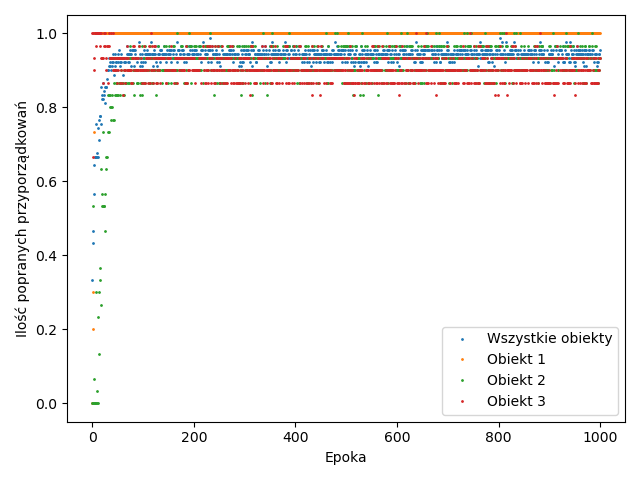
\includegraphics[width=12cm]{WykresPrzyporzadkowania5neuron3wejscia.png}
 \caption{Wykres Zmiany Jakości przyporządkowania dla 1000 epok}
 \vspace{-0.1cm}
 \label{WykresPrzyp4}
\end{figure}

\newpage

\begin{figure}[!ht]
 \centering
 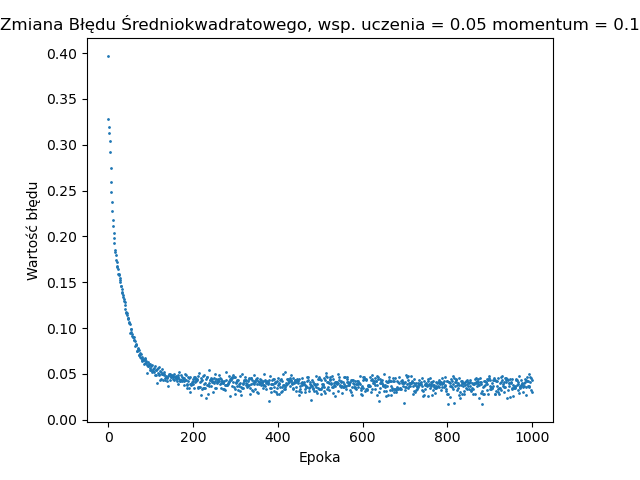
\includegraphics[width=12cm]{WykresBlad5neuron3wejscia1.png}
 \caption{Wykres Zmiany Błędu Średniokwadratowego dla 1000 epok}
 \vspace{-0.1cm}
 \label{WykresBlad4}
\end{figure}

Jak widzimy, proces nauki wygląda podobnie jak w poprzednim eksperymencie po zwiększeniu liczby neuronów.\\ Zauważamy jednak że w procesie naukii poziom przyporządkowania obiektu nr 3 nie jest już 100 procentowy.
\newpage

\begin{table}
\caption{\label{tab:tablica4} Macierz Pomyłek dla 5 neuronów i 3 wejść }
\begin{tabular}{ |p{3cm}|p{3cm}|p{2cm}|p{2cm}|p{2cm}|  }
 \hline
 & & 
 \multicolumn{3}{|c|}{Przyporządkowane Klasy} \\
 \hline

   & & Klasa 1 & Klasa 2 & Klasa 3\\
 \hline
\multirow{3}{4em}{Klasy Źródłowe}
   & Klasa 1 & 31 & 0 & 0 \\ 
   & Klasa 2 & 0 & 30 & 1 \\
   & Klasa 3 & 0 & 10 & 21 \\

 \hline
\end{tabular}
\end{table}

Nasze obawy zostają potwierdzone przez przetestowanie nauki na zbiorze testowym.\\ Sieć w aktualnym ustawieniu ma duże problemy z przyporządkowaniem Klasy 3.
\\Klasa 1 - Precision = 31 / 31, Recall = 31/31\\
Klasa 2 - Precision = 30/40 , Recall = 30/31\\
Klasa 3 - Precision = 21/22, Recall = 21 / 31\\

Ponawiamy eksperyment dla 5 neuronów lecz używamy teraz danych testowych w kolumnach 2, 3, 4.

\begin{figure}[!ht]
 \centering
 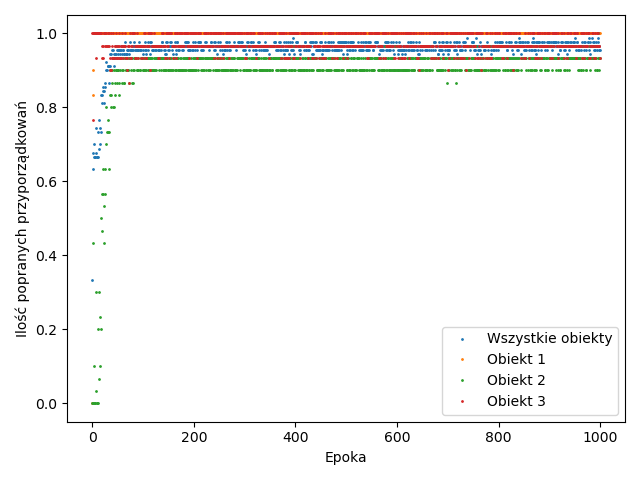
\includegraphics[width=12cm]{WykresPrzyporzadkowania5neuron3wejscia2.png}
 \caption{Wykres Zmiany Jakości przyporządkowania dla 1000 epok}
 \vspace{-0.1cm}
 \label{WykresPrzyp6}
\end{figure}

\newpage

\begin{figure}[!ht]
 \centering
 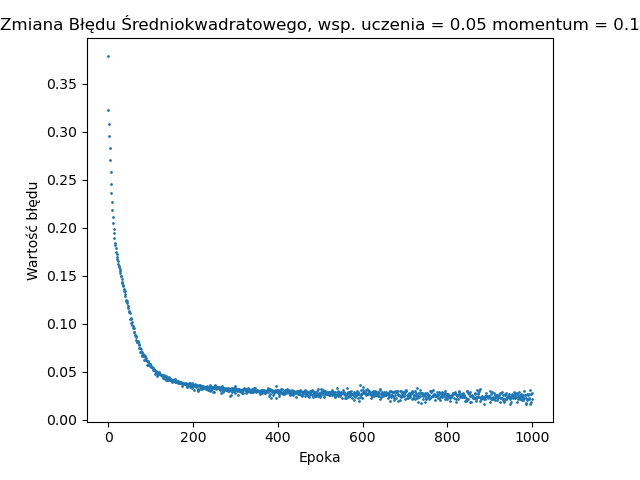
\includegraphics[width=12cm]{WykresBlad5neuron3wejscia2.png}
 \caption{Wykres Zmiany Błędu Średniokwadratowego dla 1000 epok}
 \vspace{-0.1cm}
 \label{WykresBlad6}
\end{figure}

Zauważamy, że dla tego zbioru treningowego przyporządkowanie klasy dla obiektów wydaje się przebiegać bardziej dokładnie. Błąd średniokwadratowy wydaje się być bardziej stały niż w poprzednim przypadku a wykres poprawnego przyporządkowania w kolejnych epokach wydaje się zbliżać bardziej do 100\%, zwłaszcza dla obiektu z klasy 3.

\newpage

\begin{table}
\caption{\label{tab:tablica5} Macierz Pomyłek dla 5 neuronów i 3 wejść }
\begin{tabular}{ |p{3cm}|p{3cm}|p{2cm}|p{2cm}|p{2cm}|  }
 \hline
 & & 
 \multicolumn{3}{|c|}{Przyporządkowane Klasy} \\
 \hline

   & & Klasa 1 & Klasa 2 & Klasa 3\\
 \hline
\multirow{3}{4em}{Klasy Źródłowe}
   & Klasa 1 & 31 & 0 & 0 \\ 
   & Klasa 2 & 0 & 29 & 2 \\
   & Klasa 3 & 0 & 1 & 30 \\

 \hline
\end{tabular}
\end{table}

Potwierdza to sprawdzenie na zbiorze testowym. Klasa 3 wydaje się być w tym przypadku poprawnie przyporządkowywana.
\\Klasa 1 - Precision = 31/31, Recall = 31/31\\
Klasa 2 - Precision = 29/30 , Recall = 29/31\\
Klasa 3 - Precision = 30/32, Recall = 30/ 31\\
W następnej części eksperymentu wykorzystujemy wszystkie kolumny danych poza 3cią.
\newpage

\begin{figure}[!ht]
 \centering
 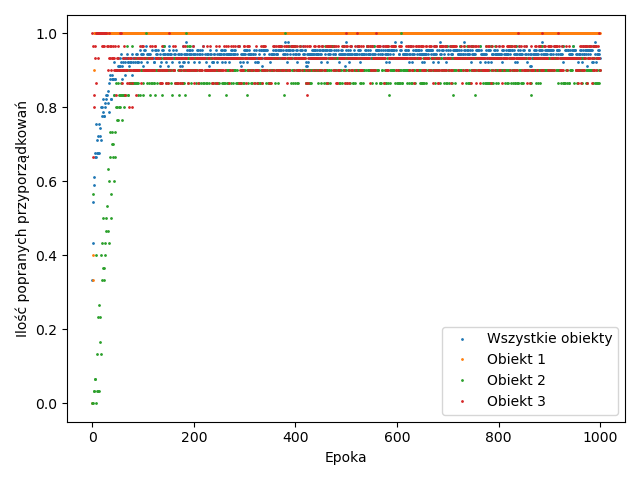
\includegraphics[width=11cm]{WykresPrzyporzadkowania5neuron3wejscia3.png}
 \caption{Wykres Zmiany Jakości przyporządkowania dla 1000 epok}
 \vspace{-0.1cm}
 \label{WykresPrzyp7}
\end{figure}


\begin{figure}[!ht]
 \centering
 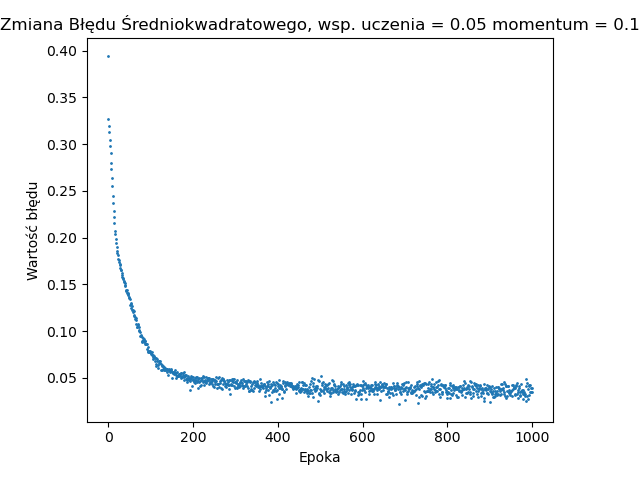
\includegraphics[width=11cm]{WykresBlad5neuron3wejscia3.png}
 \caption{Wykres Zmiany Błędu Średniokwadratowego dla 1000 epok}
 \vspace{-0.1cm}
 \label{WykresBlad7}
\end{figure}
\newpage 

\begin{table}
\caption{\label{tab:tablica6} Macierz Pomyłek dla 5 neuronów i 3 wejść }
\begin{tabular}{ |p{3cm}|p{3cm}|p{2cm}|p{2cm}|p{2cm}|  }
 \hline
 & & 
 \multicolumn{3}{|c|}{Przyporządkowane Klasy} \\
 \hline

   & & Klasa 1 & Klasa 2 & Klasa 3\\
 \hline
\multirow{3}{4em}{Klasy Źródłowe}
   & Klasa 1 & 31 & 0 & 0 \\ 
   & Klasa 2 & 0 & 31 & 0 \\
   & Klasa 3 & 0 & 6 & 25 \\

 \hline
\end{tabular}
\end{table}
Dla tego zbioru testowego pierwszy raz udało się w 100\% poprawnie zklasyfikować obiekty z klasy 2, niestety zakwalifikowalismy do niej również obiekty nie należące do niej.
\\Klasa 1 - Precision = 31/31, Recall = 31/31\\
Klasa 2 - Precision = 31/37 , Recall = 31/31\\
Klasa 3 - Precision = 25/25, Recall = 25/ 31\\
W następnej części eksperymentu będziemy korzystać z pierwszej, trzeciej oraz ostatniej kolumny zbioru treningowego.

\newpage

\begin{figure}[!ht]
 \centering
 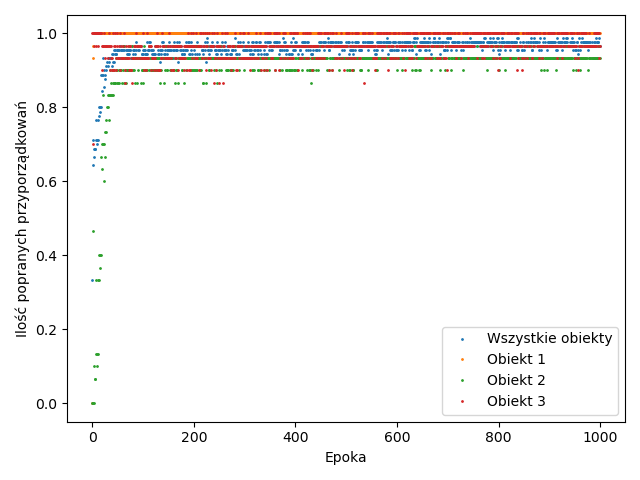
\includegraphics[width=11cm]{WykresPrzyporzadkowania5neuron3wejscia4.png}
 \caption{Wykres Zmiany Jakości przyporządkowania dla 1000 epok}
 \vspace{-0.1cm}
 \label{WykresPrzyp8}
\end{figure}


\begin{figure}[!ht]
 \centering
 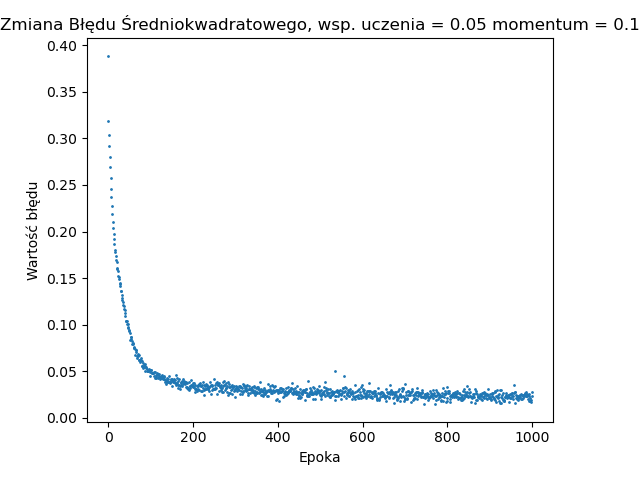
\includegraphics[width=11cm]{WykresBlad5neuron3wejscia4.png}
 \caption{Wykres Zmiany Błędu Średniokwadratowego dla 1000 epok}
 \vspace{-0.1cm}
 \label{WykresBlad8}
\end{figure}
\newpage 

\begin{table}
\caption{\label{tab:tablica7} Macierz Pomyłek dla 5 neuronów i 3 wejść }
\begin{tabular}{ |p{3cm}|p{3cm}|p{2cm}|p{2cm}|p{2cm}|  }
 \hline
 & & 
 \multicolumn{3}{|c|}{Przyporządkowane Klasy} \\
 \hline

   & & Klasa 1 & Klasa 2 & Klasa 3\\
 \hline
\multirow{3}{4em}{Klasy Źródłowe}
   & Klasa 1 & 31 & 0 & 0 \\ 
   & Klasa 2 & 0 & 28 & 3 \\
   & Klasa 3 & 0 & 0 & 31 \\

 \hline
\end{tabular}
\end{table}

Jak widzimy w tablicy, Tab. \ref{tab:tablica7}, oraz na rysunkach, Rys. \ref{WykresPrzyp8} i Rys. \ref{WykresBlad8} otrzymalismy bardzo zbliżone wyniki do tych otrzymanych dla 3 neuronów oraz 5 wejść. Możliwe , że druga kolumna zbioru treningowego nie ma wpływu na wynik klasyfikacji. Sprawdzimy to w następnym eksperymencie.
\\Klasa 1 - Precision = 31/31, Recall = 31/31\\
Klasa 2 - Precision = 28/28, Recall = 28/31\\
Klasa 3 - Precision = 31/34, Recall = 31/31\\
\newpage
\subsection {Eksperyment 3}
W tym eksperymencie zaczynamy od sprawdzenia wpływu kolumny 2 na klasyfikacje.\\W tym celu najpierw przetestujemy sieć z dwoma wejściami, odpowiednio kolumna 1 i 2 a następnie z jedym wejściem, kolumną 1.\\
Tym razem postanowiliśmy przeprowadzić eksperyment dla 20 neuronów.

\newpage

\begin{figure}[!ht]
 \centering
 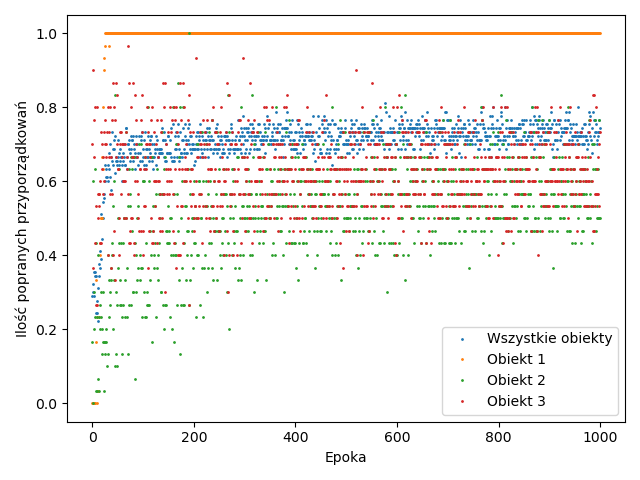
\includegraphics[width=11cm]{WykresPrzyporzadkowania20neuron2wejscia1.png}
 \caption{Wykres Zmiany Jakości przyporządkowania dla 1000 epok}
 \vspace{-0.1cm}
 \label{WykresPrzyp9}
\end{figure}


\begin{figure}[!ht]
 \centering
 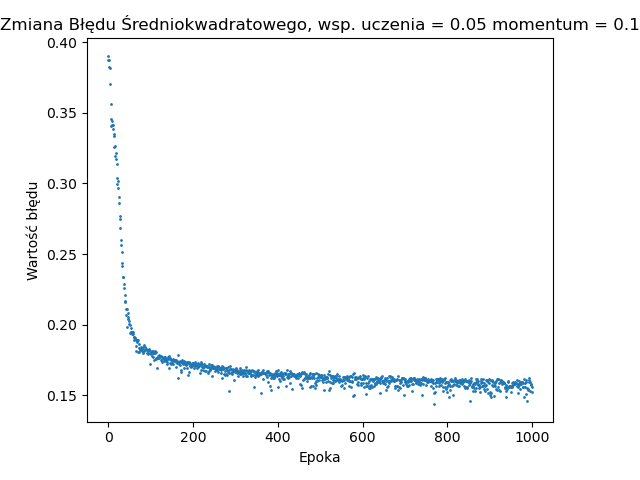
\includegraphics[width=11cm]{WykresBlad20neuron2wejscia1.png}
 \caption{Wykres Zmiany Błędu Średniokwadratowego dla 1000 epok}
 \vspace{-0.1cm}
 \label{WykresBlad9}
\end{figure}
\newpage 


\begin{table}
\caption{\label{tab:tablica8} Macierz Pomyłek dla 20 neuronów i 2 wejść }
\begin{tabular}{ |p{3cm}|p{3cm}|p{2cm}|p{2cm}|p{2cm}|  }
 \hline
 & & 
 \multicolumn{3}{|c|}{Przyporządkowane Klasy} \\
 \hline

   & & Klasa 1 & Klasa 2 & Klasa 3\\
 \hline
\multirow{3}{4em}{Klasy Źródłowe}
   & Klasa 1 & 30 & 1 & 0 \\ 
   & Klasa 2 & 0 & 24 & 7 \\
   & Klasa 3 & 0 & 10 & 21 \\

 \hline
\end{tabular}
\end{table}
Jak widzimy, klasyfikacja dla obiektu 1 w zbiorze testowym przebiega poprawnie w 100\% przypadków, jednak klasyfikacja kolejnych klas pozostawia wiele do życzenia. \\
Jak widzimy z tabeli, Tab \ref{tab:tablica8}, jest to pierwszy przypadek w którym obiekty klasy 1 nie zostały perfekcyjnie zklasyfikowane, mimo że na zbiorze testowym wydawały się one być idealnie klasyfikowane. Klasyfikacja obiektów pozostałych klas pozostawia wiele do życzenia.
\\Klasa 1 - Precision = 30/30, Recall = 30/31\\
Klasa 2 - Precision = 24/35, Recall = 24/31\\
Klasa 3 - Precision = 21/28, Recall = 21/31\\
 Powtarzamy próbę dla 1 wejścia.

\newpage

\begin{figure}[!ht]
 \centering
 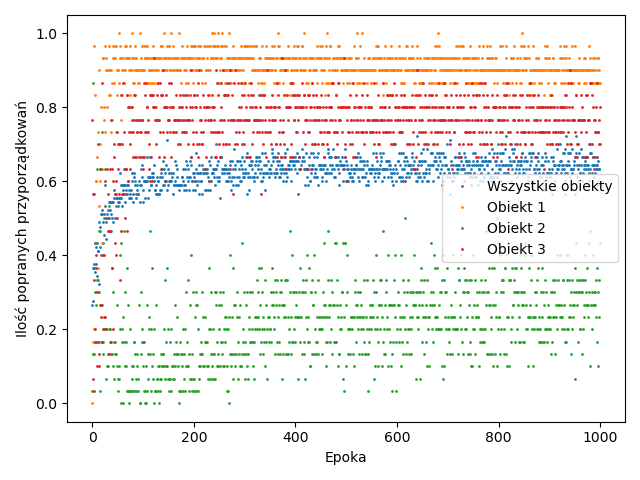
\includegraphics[width=11cm]{WykresPrzyporzadkowania20neuron1wejscia1.png}
 \caption{Wykres Zmiany Jakości przyporządkowania dla 1000 epok}
 \vspace{-0.1cm}
 \label{WykresPrzyp10}
\end{figure}


\begin{figure}[!ht]
 \centering
 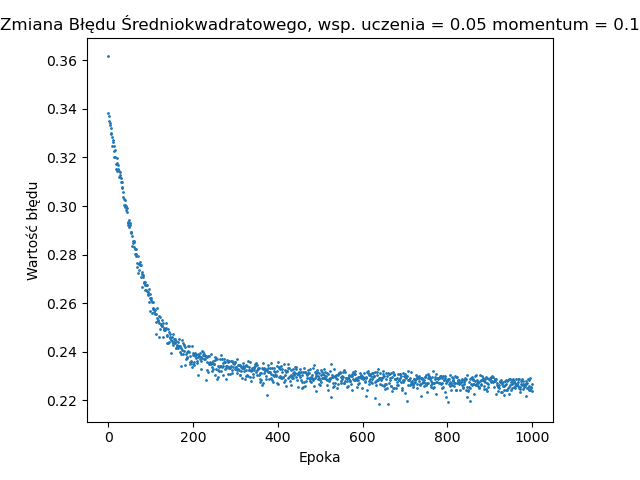
\includegraphics[width=11cm]{WykresBlad20neuron1wejscia1.png}
 \caption{Wykres Zmiany Błędu Średniokwadratowego dla 1000 epok}
 \vspace{-0.1cm}
 \label{WykresBlad10}
\end{figure}
\newpage 

\begin{table}
\caption{\label{tab:tablica9} Macierz Pomyłek dla 20 neuronów i 1 wejścia }
\begin{tabular}{ |p{3cm}|p{3cm}|p{2cm}|p{2cm}|p{2cm}|  }
 \hline
 & & 
 \multicolumn{3}{|c|}{Przyporządkowane Klasy} \\
 \hline

   & & Klasa 1 & Klasa 2 & Klasa 3\\
 \hline
\multirow{3}{4em}{Klasy Źródłowe}
   & Klasa 1 & 31 & 0 & 0 \\ 
   & Klasa 2 & 7 & 13 & 11 \\
   & Klasa 3 & 0 & 5 & 26 \\

 \hline
\end{tabular}
\end{table}
\newpage
Od razu możemy zauważyć, że klasyfikacja, poza obiektami klasy 1, nie przebiega sprawnie. Klasyfikacja obiektów z klasy 2 wogole nie przebiega a także klasyfikacja obiektów z klasy 3 pozostawia wiele do życzenia. Można śmiało założyć, że pierwsza kolumna jest najbardziej charakterystyczna dla obiektów klasy 1, a do wykrycia obiektów klasy 2 prawdopodobnie mozna ją całkowicie pominąć.
\\Klasa 1 - Precision = 31/38, Recall = 31/31\\
Klasa 2 - Precision = 13/18, Recall = 13/31\\
Klasa 3 - Precision = 26/37, Recall = 26/31\\
Jak widzimy z macierzy pomyłek dla zbioru testowego klasa 1 była rozpoznawana idealnie. Obiekty jednak klasy 2 były zupełnie nie możliwe dla rozpoznania dla sieci i zostały przypisane można powiedzieć że losowo, a klasyfikacja obiektów klasy 3 też nie była zbyt dobra.

\newpage
Kontynuujemy eksperyment sprawdzając kolejne 2 kolumny danych w sieci z dwoma wejściami. Będą to kolumna druga i trzecia.\\Eksperyment przeprowadzamy dla 10 neuronów w warstwie ukrytej.

\begin{figure}[!ht]
 \centering
 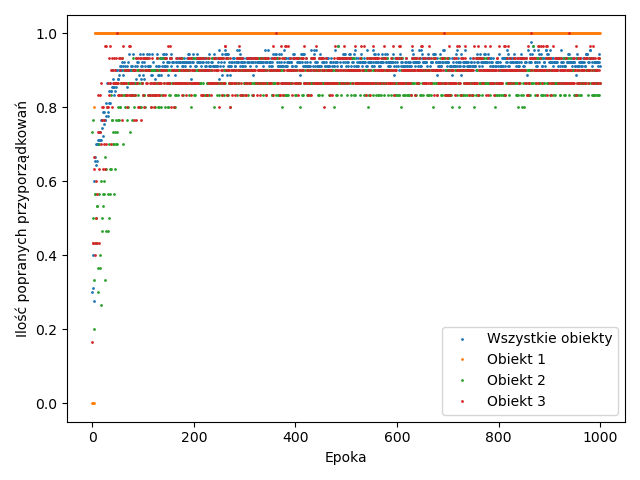
\includegraphics[width=11cm]{WykresPrzyporzadkowania10neuron2wejscia1.png}
 \caption{Wykres Zmiany Jakości przyporządkowania dla 1000 epok}
 \vspace{-0.1cm}
 \label{WykresPrzyp11}
\end{figure}

\newpage

\begin{figure}[!ht]
 \centering
 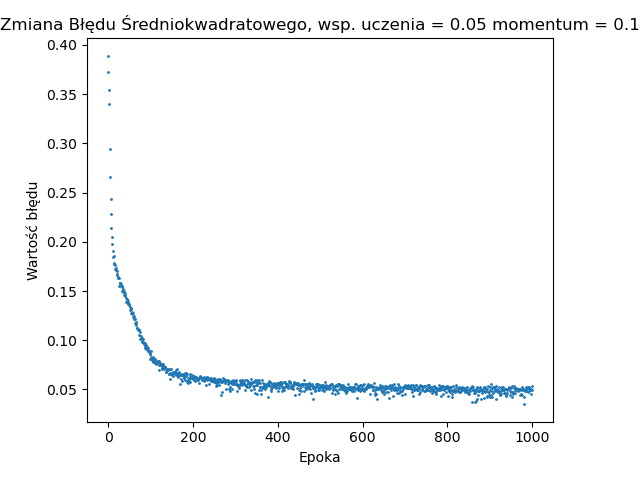
\includegraphics[width=11cm]{WykresBlad10neuron2wejscia1.png}
 \caption{Wykres Zmiany Błędu Średniokwadratowego dla 1000 epok}
 \vspace{-0.1cm}
 \label{WykresBlad11}
\end{figure}

Jak możemy łatwo zobaczyć z wykresów na rysunkach, Rys. \ref{WykresPrzyp11} i Rys. \ref{WykresBlad11}, jakość przyporządkowania klas w tym etapie treningowym jest o wiele większa niż dla poprzednio wybranych dwu kolumn danych. Błąd średniokwadratowy jest blisko 3 razy mniejszy i poziom klasyfikacji w zbiorze treningowym jest bardzo wysoki.\\
\newpage
\begin{table}
\caption{\label{tab:tablica10} Macierz Pomyłek dla 10 neuronów i 2 wejść}
\begin{tabular}{ |p{3cm}|p{3cm}|p{2cm}|p{2cm}|p{2cm}|  }
 \hline
 & & 
 \multicolumn{3}{|c|}{Przyporządkowane Klasy} \\
 \hline

   & & Klasa 1 & Klasa 2 & Klasa 3\\
 \hline
\multirow{3}{4em}{Klasy Źródłowe}
   & Klasa 1 & 31 & 0 & 0 \\ 
   & Klasa 2 & 0 & 26 & 5 \\
   & Klasa 3 & 0 & 1 & 30 \\

 \hline
\end{tabular}
\end{table}
 
Wyniki klasyfikacji na zbiorze testowym okazują się bardzo przyzwoite. Wszystkie obiekty klasy 1 zostały poprawnie przyporządkowane, a i klasyfikacja dla obiektów klasy 2 i 3 można ocenić na 'dobrą'.
\\Klasa 1 - Precision = 31/31, Recall = 31/31\\
Klasa 2 - Precision = 26/27, Recall = 16/31\\
Klasa 3 - Precision = 30/35, Recall = 30/31\\
\newpage
Kontynuujemy eksperyment dla 2 ostatnich kolumn danych. Pozostałe ustawienia identyczne jak w poprzednim eksperymencie.

\begin{figure}[!ht]
 \centering
 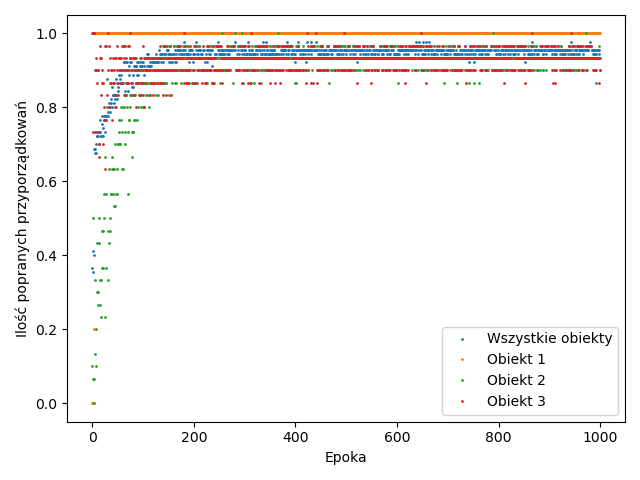
\includegraphics[width=11cm]{WykresPrzyporzadkowania10neuron2wejscia2.png}
 \caption{Wykres Zmiany Jakości przyporządkowania dla 1000 epok}
 \vspace{-0.1cm}
 \label{WykresPrzyp12}
\end{figure}

\newpage

\begin{figure}[!ht]
 \centering
 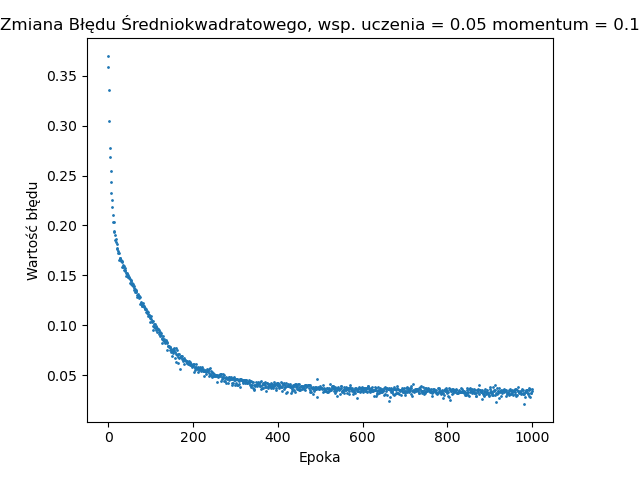
\includegraphics[width=11cm]{WykresBlad10neuron2wejscia2.png}
 \caption{Wykres Zmiany Błędu Średniokwadratowego dla 1000 epok}
 \vspace{-0.1cm}
 \label{WykresBlad12}
\end{figure}

Wyniki bardzo podobne jak przy poprzedniej części eksperymentu, pozostawiamy bez komentarza.

\newpage
\begin{table}
\caption{\label{tab:tablica11} Macierz Pomyłek dla 10 neuronów i 2 wejść}
\begin{tabular}{ |p{3cm}|p{3cm}|p{2cm}|p{2cm}|p{2cm}|  }
 \hline
 & & 
 \multicolumn{3}{|c|}{Przyporządkowane Klasy} \\
 \hline

   & & Klasa 1 & Klasa 2 & Klasa 3\\
 \hline
\multirow{3}{4em}{Klasy Źródłowe}
   & Klasa 1 & 31 & 0 & 0 \\ 
   & Klasa 2 & 0  & 28 & 3 \\
   & Klasa 3 & 0  & 3   & 28 \\

 \hline
\end{tabular}
\end{table}
Również tutaj bardzo podobne wyniki pozostawiamy bez komentarza.
\\Klasa 1 - Precision = 31/31, Recall = 31/31\\
Klasa 2 - Precision = 28/31, Recall = 28/31\\
Klasa 3 - Precision = 28/31, Recall = 28/31\\
\newpage
Kolejna część eksperymentu, tym razem pierwsza i czwarta kolumna danych.

\begin{figure}[!ht]
 \centering
 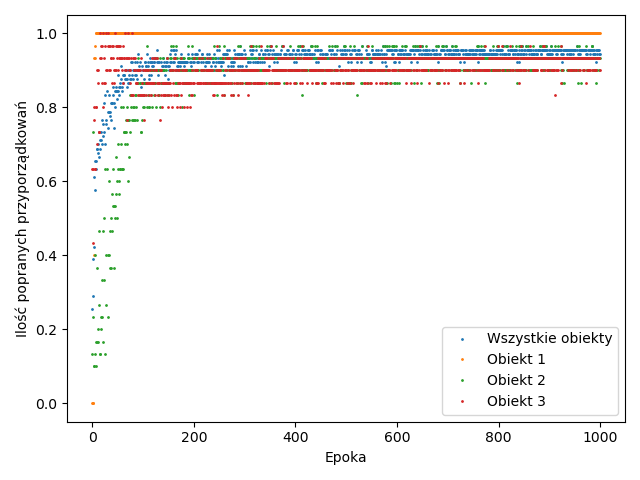
\includegraphics[width=11cm]{WykresPrzyporzadkowania10neuron2wejscia3.png}
 \caption{Wykres Zmiany Jakości przyporządkowania dla 1000 epok}
 \vspace{-0.1cm}
 \label{WykresPrzyp13}
\end{figure}

\newpage

\begin{figure}[!ht]
 \centering
 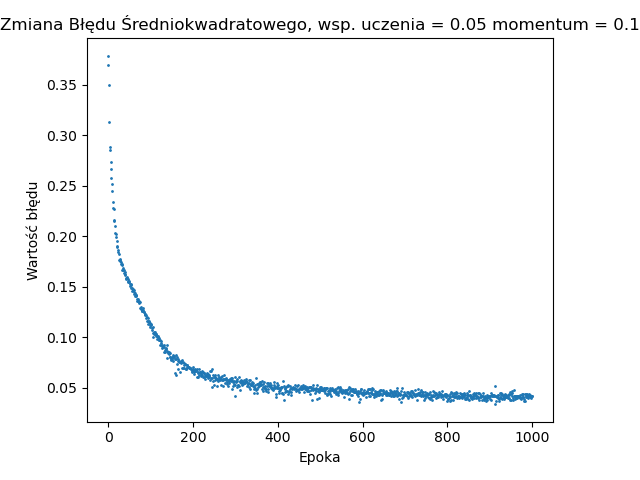
\includegraphics[width=11cm]{WykresBlad10neuron2wejscia3.png}
 \caption{Wykres Zmiany Błędu Średniokwadratowego dla 1000 epok}
 \vspace{-0.1cm}
 \label{WykresBlad13}
\end{figure}


\newpage
\begin{table}
\caption{\label{tab:tablica12} Macierz Pomyłek dla 10 neuronów i 2 wejść}
\begin{tabular}{ |p{3cm}|p{3cm}|p{2cm}|p{2cm}|p{2cm}|  }
 \hline
 & & 
 \multicolumn{3}{|c|}{Przyporządkowane Klasy} \\
 \hline

   & & Klasa 1 & Klasa 2 & Klasa 3\\
 \hline
\multirow{3}{4em}{Klasy Źródłowe}
   & Klasa 1 & 31 & 0 & 0 \\ 
   & Klasa 2 & 0  & 27 & 4 \\
   & Klasa 3 & 0  & 4   & 27 \\
 \hline
\end{tabular}
\end{table}
Wyniki prawie identyczne jak poprzednie, pozostawiamy bez komentarza.
\\Klasa 1 - Precision = 31/31, Recall = 31/31\\
Klasa 2 - Precision = 27/31, Recall = 27/31\\
Klasa 3 - Precision = 27/31, Recall = 27/31\\
\newline
Kolejna część eksperymentu, analizujemy kolumny nr 1 oraz 3

\begin{figure}[!ht]
 \centering
 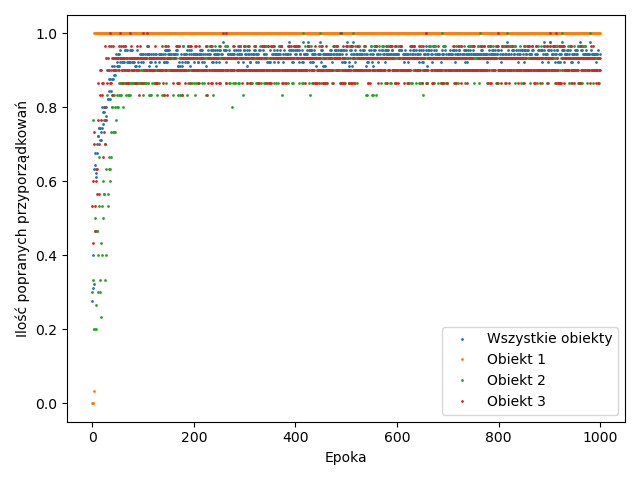
\includegraphics[width=11cm]{WykresPrzyporzadkowania10neuron2wejscia4.png}
 \caption{Wykres Zmiany Jakości przyporządkowania dla 1000 epok}
 \vspace{-0.1cm}
 \label{WykresPrzyp14}
\end{figure}

\newpage

\begin{figure}[!ht]
 \centering
 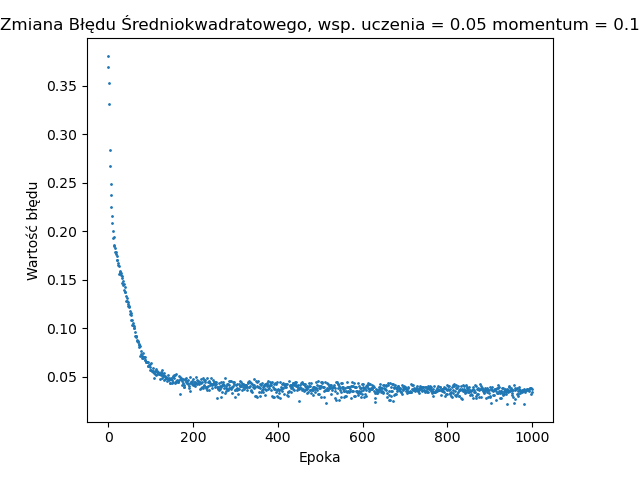
\includegraphics[width=11cm]{WykresBlad10neuron2wejscia4.png}
 \caption{Wykres Zmiany Błędu Średniokwadratowego dla 1000 epok}
 \vspace{-0.1cm}
 \label{WykresBlad14}
\end{figure}


\begin{table}
\caption{\label{tab:tablica13} Macierz Pomyłek dla 10 neuronów i 2 wejść}
\begin{tabular}{ |p{3cm}|p{3cm}|p{2cm}|p{2cm}|p{2cm}|  }
 \hline
 & & 
 \multicolumn{3}{|c|}{Przyporządkowane Klasy} \\
 \hline

   & & Klasa 1 & Klasa 2 & Klasa 3\\
 \hline
\multirow{3}{4em}{Klasy Źródłowe}
   & Klasa 1 & 31 & 0 & 0 \\ 
   & Klasa 2 & 0  & 26 & 5 \\
   & Klasa 3 & 0  & 2   & 29 \\
 \hline
\end{tabular}
\end{table}

Znowu, jak w kilku poprzednich próbach Klasa 1 dopasowana perfekcyjnie, a klasy 2 i 3 w bardzo wysokim stopniu. Łącznie 86 z 93 obiektów zostało odpowiednio przyporządkowanych. 
\\Klasa 1 - Precision = 31/31, Recall = 31/31\\
Klasa 2 - Precision = 26/28, Recall = 26/31\\
Klasa 3 - Precision = 29/35, Recall = 29/31\\

\newpage

Ostatnia próba dla 2 kolumn danych, korzystamy z kolumn 2 i 4.

\begin{figure}[!ht]
 \centering
 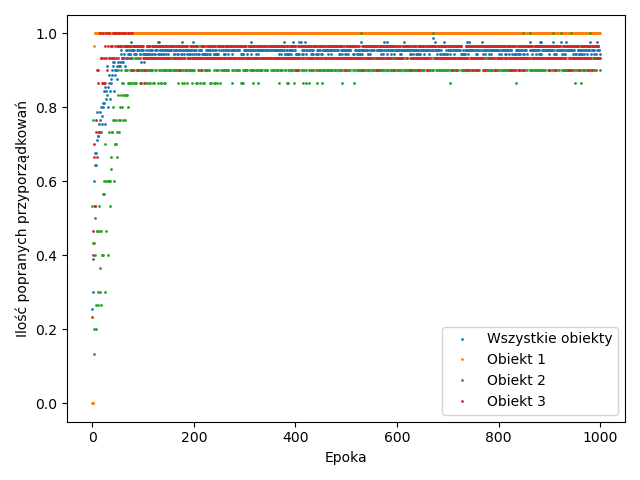
\includegraphics[width=11cm]{WykresPrzyporzadkowania10neuron2wejscia5.png}
 \caption{Wykres Zmiany Jakości przyporządkowania dla 1000 epok}
 \vspace{-0.1cm}
 \label{WykresPrzyp15}
\end{figure}

\newpage

\begin{figure}[!ht]
 \centering
 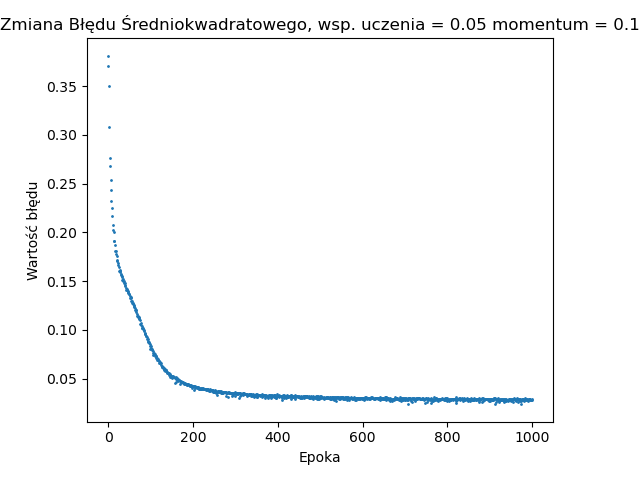
\includegraphics[width=11cm]{WykresBlad10neuron2wejscia5.png}
 \caption{Wykres Zmiany Błędu Średniokwadratowego dla 1000 epok}
 \vspace{-0.1cm}
 \label{WykresBlad15}
\end{figure}

\begin{table}
\caption{\label{tab:tablica14} Macierz Pomyłek dla 20 neuronów i 2 wejść}
\begin{tabular}{ |p{3cm}|p{3cm}|p{2cm}|p{2cm}|p{2cm}|  }
 \hline
 & & 
 \multicolumn{3}{|c|}{Przyporządkowane Klasy} \\
 \hline

   & & Klasa 1 & Klasa 2 & Klasa 3\\
 \hline
\multirow{3}{4em}{Klasy Źródłowe}
   & Klasa 1 & 31 & 0 & 0 \\ 
   & Klasa 2 & 0  & 30 & 1 \\
   & Klasa 3 & 0  & 3  & 28 \\
 \hline
\end{tabular}
\end{table}

Zauważalnie lepsze przyporządkowanie klas niż w poprzednich próbach.\\Zarówno błąd średniokwadratowy na próbie treningowej jak i przyporządkowanie na próbie treningowej jak i testowej wypada 'lepiej' niż w żadnej innej próbie dla 2 kolumn danych.
\\Klasa 1 - Precision = 31/31, Recall = 31/31\\
Klasa 2 - Precision = 30/33, Recall = 30/31\\
Klasa 3 - Precision = 28/29, Recall = 28/31\\

\newpage
Powtórzylismy próbę dla 1 neurona.



\begin{figure}[!ht]
 \centering
 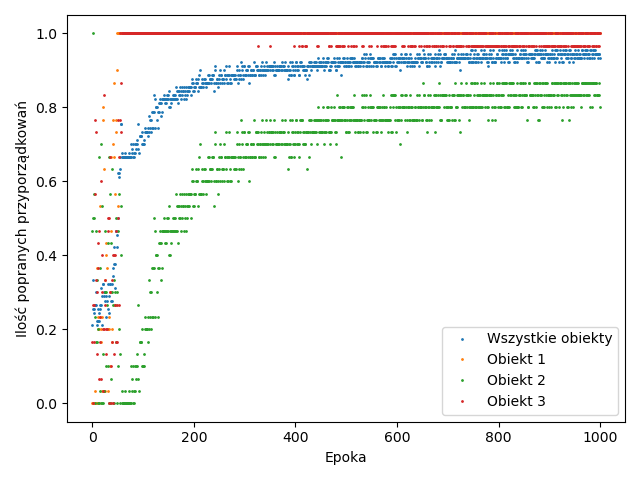
\includegraphics[width=11cm]{WykresPrzyporzadkowania1neuron2wejscia.png}
 \caption{Wykres Zmiany Jakości przyporządkowania dla 1000 epok}
 \vspace{-0.1cm}
 \label{WykresPrzyp16}
\end{figure}

\newpage

\begin{figure}[!ht]
 \centering
 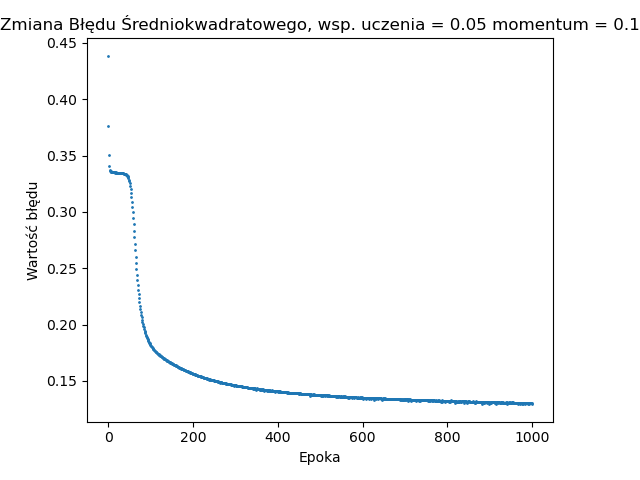
\includegraphics[width=11cm]{WykresBlad1neuron2wejscia.png}
 \caption{Wykres Zmiany Błędu Średniokwadratowego dla 1000 epok}
 \vspace{-0.1cm}
 \label{WykresBlad16}
\end{figure}

\begin{table}
\caption{\label{tab:tablica16} Macierz Pomyłek dla 1 neurona i 2 wejść}
\begin{tabular}{ |p{3cm}|p{3cm}|p{2cm}|p{2cm}|p{2cm}|  }
 \hline
 & & 
 \multicolumn{3}{|c|}{Przyporządkowane Klasy} \\
 \hline

   & & Klasa 1 & Klasa 2 & Klasa 3\\
 \hline
\multirow{3}{4em}{Klasy Źródłowe}
   & Klasa 1 & 31 & 0 & 0 \\ 
   & Klasa 2 & 0  & 27 & 4 \\
   & Klasa 3 & 0  & 3  & 28 \\
 \hline
\end{tabular}
\end{table}

Wyniki okazały się bardzo dobre jak na użycie tylko 1 neuronu. Błąd zaróno podczas treningu jak i ilość pomyłek na próbie testowej okazały się zadziwiająco niskie.
\\Klasa 1 - Precision = 31/31, Recall = 31/31\\
Klasa 2 - Precision = 27/30, Recall = 27/31\\
Klasa 3 - Precision = 28/32, Recall = 28/31\\

\newpage
\subsection {Eksperyment 4}

W tym Segmencie sprawozdania testujemy sieć neuronową z jedynie jednym wejściem.\\ Zaczynamy od drugiej kolumny danych ponieważ pierwszą przetestowaliśmy już wcześniej w Eksperymencie 3.\\ Eksperymenty przeprowadzamy dla 5 neuronów w warstwie ukrytej.

\begin{figure}[!ht]
 \centering
 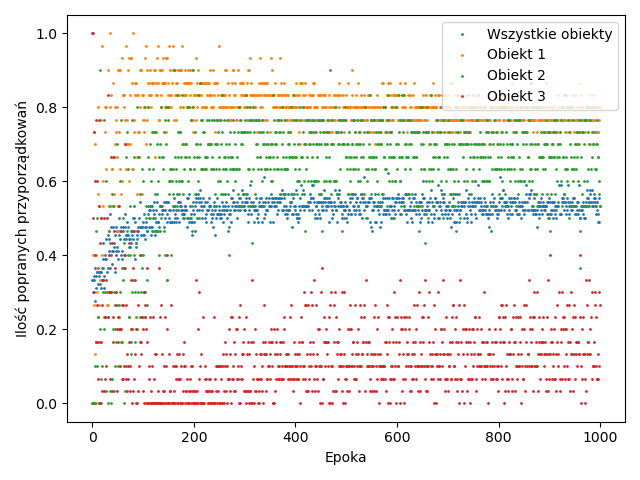
\includegraphics[width=11cm]{WykresPrzyporzadkowania5neuron1wejscia.png}
 \caption{Wykres Zmiany Jakości przyporządkowania dla 1000 epok}
 \vspace{-0.1cm}
 \label{WykresPrzyp18}
\end{figure}

\newpage

\begin{figure}[!ht]
 \centering
 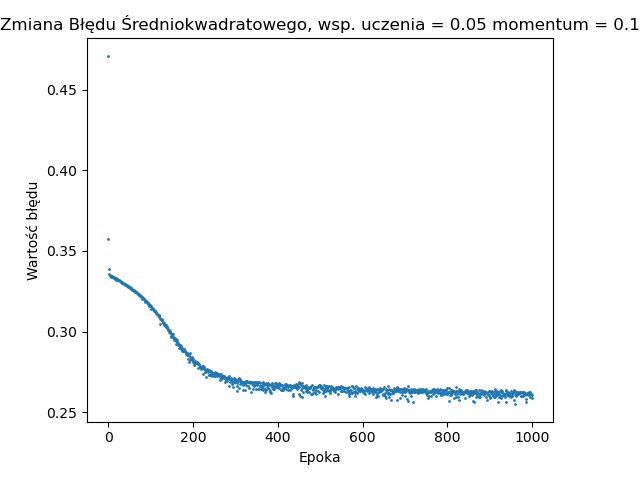
\includegraphics[width=11cm]{WykresBlad5neuron1wejscia1.png}
 \caption{Wykres Zmiany Błędu Średniokwadratowego dla 1000 epok}
 \vspace{-0.1cm}
 \label{WykresBlad18}
\end{figure}

\begin{table}
\caption{\label{tab:tablica17} Macierz Pomyłek dla 5 neuronów  i 1 wejścia}
\begin{tabular}{ |p{3cm}|p{3cm}|p{2cm}|p{2cm}|p{2cm}|  }
 \hline
 & & 
 \multicolumn{3}{|c|}{Przyporządkowane Klasy} \\
 \hline

   & & Klasa 1 & Klasa 2 & Klasa 3\\
 \hline
\multirow{3}{4em}{Klasy Źródłowe}
   & Klasa 1 & 20 & 4 & 7 \\ 
   & Klasa 2 & 1  & 28 & 2 \\
   & Klasa 3 & 5  & 19  & 7 \\
 \hline
\end{tabular}
\end{table}
Zgodnie z naszymi oczekiwaniami nauka dla jednego wejścia postępuje 'najgorzej'. Na wykresie przyporządkowania w trakcie treningu widać 'chaos'. Sieć najlepiej nauczyła się rozpoznawać obiekty z klasy drugiej, gorzej klasy pierwszej, a obiekty klasy 3 nie nauczyła się klasyfikować wogóle. Błąd średniokwadratowy najwyższy z wszystkich prób dotychczas.
\\Klasa 1 - Precision = 20/31, Recall = 20/31\\
Klasa 2 - Precision = 28/51, Recall = 28/31\\
Klasa 3 - Precision = 07/16, Recall = 7/31\\

\newpage

Powtarzamy eksperyment dla kolejnej kolumny danych (3)

\begin{figure}[!ht]
 \centering
 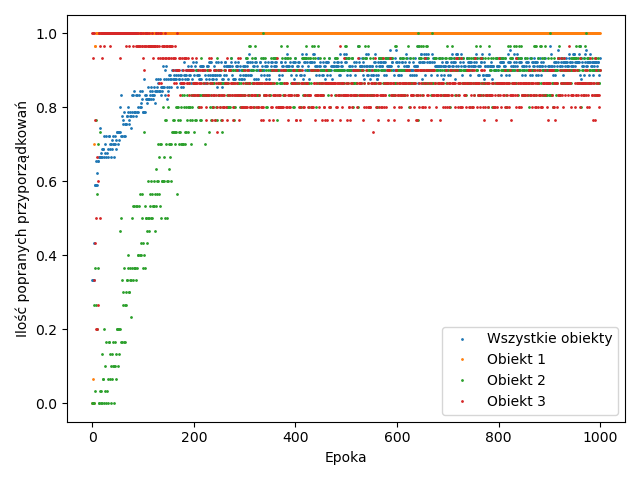
\includegraphics[width=11cm]{WykresPrzyporzadkowania5neuron1wejscia2.png}
 \caption{Wykres Zmiany Jakości przyporządkowania dla 1000 epok}
 \vspace{-0.1cm}
 \label{WykresPrzyp19}
\end{figure}

\newpage

\begin{figure}[!ht]
 \centering
 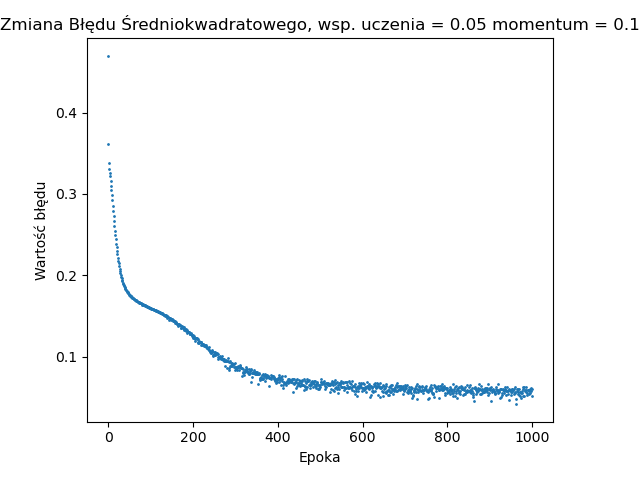
\includegraphics[width=11cm]{WykresBlad5neuron1wejscia2.png}
 \caption{Wykres Zmiany Błędu Średniokwadratowego dla 1000 epok}
 \vspace{-0.1cm}
 \label{WykresBlad19}
\end{figure}

\begin{table}
\caption{\label{tab:tablica18} Macierz Pomyłek dla 5 neuronów  i 1 wejścia}
\begin{tabular}{ |p{3cm}|p{3cm}|p{2cm}|p{2cm}|p{2cm}|  }
 \hline
 & & 
 \multicolumn{3}{|c|}{Przyporządkowane Klasy} \\
 \hline

   & & Klasa 1 & Klasa 2 & Klasa 3\\
 \hline
\multirow{3}{4em}{Klasy Źródłowe}
   & Klasa 1 & 31 & 0 & 0 \\ 
   & Klasa 2 & 0  & 28 & 3 \\
   & Klasa 3 & 0  & 2  & 29 \\
 \hline
\end{tabular}
\end{table}

Zaskakujący, nie spodziewany, wynik dla trzeciej kolumny danych. Mimo tylko jednego wejścia klasyfikacja może być określona jako 'dobra'. Błąd średniokwadratowy na zbiorze treningowym osiągnął niską wartość około 0.05, a w zbiorze testowym poprawnie przyporządkowano 88 z 93 klas. Okazuje się, że przy dobrym doborze danych treningowych nawet z 1 wejściem da się w dobrym stopniu zklasyfikować klasy.
\\Klasa 1 - Precision = 31/31, Recall = 31/31\\
Klasa 2 - Precision = 28/30, Recall = 28/31\\
Klasa 3 - Precision = 29/32, Recall = 29/31\\

\newpage

Powtarzamy eksperyment dla ostatniej kolumny danych

\begin{figure}[!ht]
 \centering
 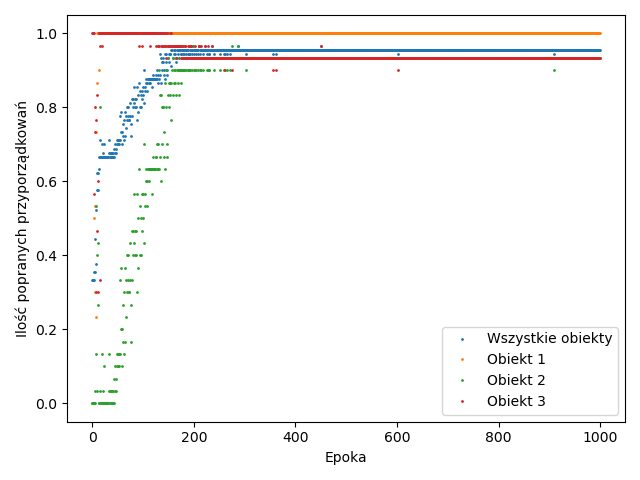
\includegraphics[width=11cm]{WykresPrzyporzadkowania5neuron1wejscia3.png}
 \caption{Wykres Zmiany Jakości przyporządkowania dla 1000 epok}
 \vspace{-0.1cm}
 \label{WykresPrzyp20}
\end{figure}

\newpage

\begin{figure}[!ht]
 \centering
 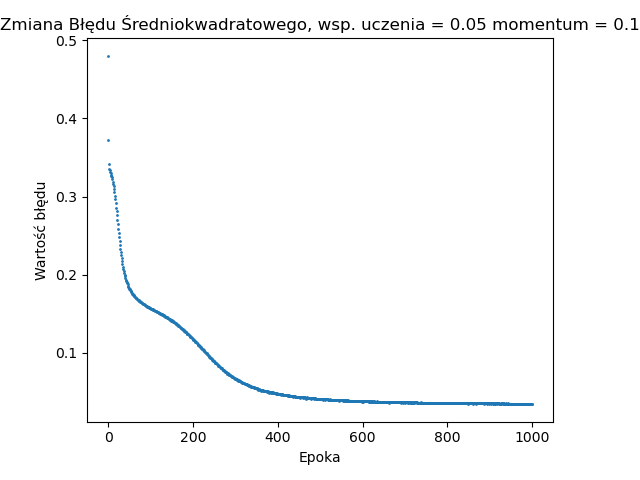
\includegraphics[width=11cm]{WykresBlad5neuron1wejscia3.png}
 \caption{Wykres Zmiany Błędu Średniokwadratowego dla 1000 epok}
 \vspace{-0.1cm}
 \label{WykresBlad20}
\end{figure}

\begin{table}
\caption{\label{tab:tablica19} Macierz Pomyłek dla 5 neuronów  i 1 wejścia}
\begin{tabular}{ |p{3cm}|p{3cm}|p{2cm}|p{2cm}|p{2cm}|  }
 \hline
 & & 
 \multicolumn{3}{|c|}{Przyporządkowane Klasy} \\
 \hline

   & & Klasa 1 & Klasa 2 & Klasa 3\\
 \hline
\multirow{3}{4em}{Klasy Źródłowe}
   & Klasa 1 & 31 & 0 & 0 \\ 
   & Klasa 2 & 0  & 28 & 3 \\
   & Klasa 3 & 0  & 2  & 29 \\
 \hline
\end{tabular}
\end{table}

Ponownie zaskakująco dobry wynik klasyfikacji, jedynie 5 z 93 obiektów w zestawie testowym nie zostało dobrze przyporządkowane. Błąd średniokwadratowy na zbiorze treningowym osiągnął okolice 0.03, co czyni go jednym z najniższych w traktcie naszych eksperymentów.
\\Klasa 1 - Precision = 31/31, Recall = 31/31\\
Klasa 2 - Precision = 28/30, Recall = 28/31\\
Klasa 3 - Precision = 29/32, Recall = 29/31\\
\newpage
\subsection {Eksperyment 5}

Analizujemy wpływ momentum i współczynniku uczenia na naukę.\\ Wzorujemy się na ustawieniach z konca poprzedniego eksperymentu, więc 1 wejście i 5 neuronów w warstwie ukrytej.

\begin{figure}[!ht]
 \centering
 \includegraphics[width=11cm]{Wykreswspuczenia.png}
 \caption{Wykres Zmiany Jakości przyporządkowania dla 1000 epok}
 \vspace{-0.1cm}
 \label{WykresPrzyp20}
\end{figure}

\newpage

\begin{figure}[!ht]
 \centering
 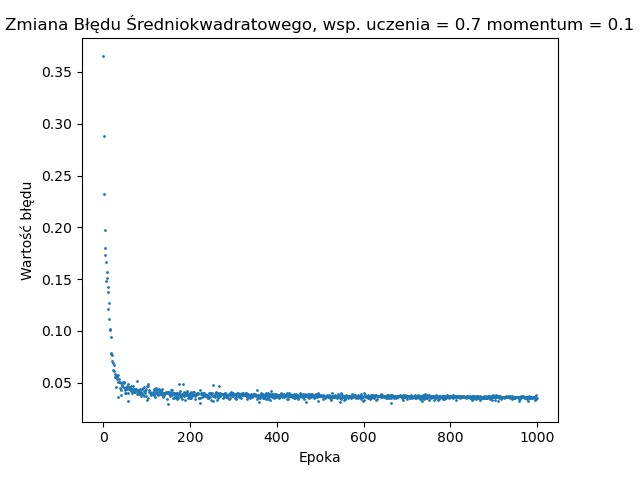
\includegraphics[width=11cm]{bladwspUczenia.png}
 \caption{Wykres Zmiany Błędu Średniokwadratowego dla 1000 epok}
 \vspace{-0.1cm}
 \label{WykresBlad20}
\end{figure}

\begin{table}
\caption{\label{tab:tablica19} Macierz Pomyłek dla 5 neuronów  i 1 wejścia}
\begin{tabular}{ |p{3cm}|p{3cm}|p{2cm}|p{2cm}|p{2cm}|  }
 \hline
 & & 
 \multicolumn{3}{|c|}{Przyporządkowane Klasy} \\
 \hline

   & & Klasa 1 & Klasa 2 & Klasa 3\\
 \hline
\multirow{3}{4em}{Klasy Źródłowe}
   & Klasa 1 & 31 & 0 & 0 \\ 
   & Klasa 2 & 0  & 29 & 2 \\
   & Klasa 3 & 0  & 4  & 27 \\
 \hline
\end{tabular}
\end{table}
Drastyczna zmiana współczynniku uczenia nie miała dużego wpływu na postęp nauki.
\\Klasa 1 - Precision = 31/31, Recall = 31/31\\
Klasa 2 - Precision = 29/33, Recall = 29/31\\
Klasa 3 - Precision = 27/29, Recall = 27/31\\
\newpage

\begin{figure}[!ht]
 \centering
 \includegraphics[width=11cm]{Wykreswspuczenia.png}
 \caption{Wykres Zmiany Jakości przyporządkowania dla 1000 epok}
 \vspace{-0.1cm}
 \label{WykresPrzyp20}
\end{figure}

\newpage

\begin{figure}[!ht]
 \centering
 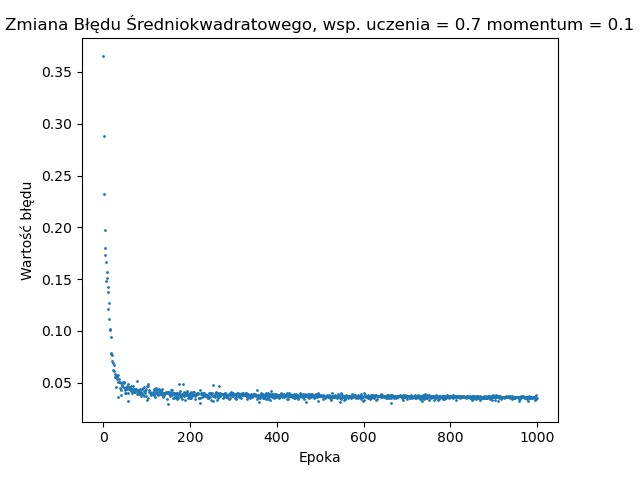
\includegraphics[width=11cm]{bladwspUczenia.png}
 \caption{Wykres Zmiany Błędu Średniokwadratowego dla 1000 epok}
 \vspace{-0.1cm}
 \label{WykresBlad20}
\end{figure}

\begin{table}
\caption{\label{tab:tablica19} Macierz Pomyłek dla 5 neuronów  i 1 wejścia}
\begin{tabular}{ |p{3cm}|p{3cm}|p{2cm}|p{2cm}|p{2cm}|  }
 \hline
 & & 
 \multicolumn{3}{|c|}{Przyporządkowane Klasy} \\
 \hline

   & & Klasa 1 & Klasa 2 & Klasa 3\\
 \hline
\multirow{3}{4em}{Klasy Źródłowe}
   & Klasa 1 & 31 & 0 & 0 \\ 
   & Klasa 2 & 0  & 29 & 2 \\
   & Klasa 3 & 0  & 4  & 27 \\
 \hline
\end{tabular}
\end{table}
Również drastyczna zmiana momentum nie wpłyneła na postępy nauki sieci.
\\Klasa 1 - Precision = 31/31, Recall = 31/31\\
Klasa 2 - Precision = 29/33, Recall = 29/31\\
Klasa 3 - Precision = 27/29, Recall = 27/31\\
\newpage


\newpage
\section {Wnioski}

Zgodnie z naszymi oczekiwaniami najlepszy wynik otrzymalismy dla 4 wejść i dużej ilości neuronów. Mimo to zaskoczyło nas jak dobrze sieć potrafi sobie poradzić przy niskiej ilości neuronów i wejść, jeżeli dobrze dobierzemy dane wejściowe. Okazuje się że najlepszymi danymi są te znajdujące się w 3 i 4 kolumnie danych treningowych, pozwoliły nam one najlepiej odszyfrować klasy obiektów, nawet przy 1 wejściu i niskiej ilości neuronów.\\ Dla większości kombinacji siec potrzebowała około 200 epok do nauki. Po tym okresie wartości błędu średniokwadratowego i ilość poprawnie rozpoznanych obiektów nie zmieniały się już o zauważalne ilości.



%%%%%%%%%%%%%%%%%%%%%%%%%%%%%%%%%%%%%%%%%%%%%%%%%%%%%%%%%%%%%%%%%%%%%%%%%%%%%%%%%%%%%%%%%%%%%%%%%%%%%%%%%%%%%%%%%
% PODROZDZIA� PT. EKSPERYMENT NR 1 
%%%%%%%%%%%%%%%%%%%%%%%%%%%%%%%%%%%%%%%%%%%%%%%%%%%%%%%%%%%%%%%%%%%%%%%%%%%%%%%%%%%%%%%%%%%%%%%%%%%%%%%%%%%%%%%%%




%%%%%%%%%%%%%%%%%%%%%%%%%%%%%%%%%%%%%%%%%%%%%%%%%%%%%%%%%%%%%%%%%%%%%%%%%%%%%%%%%%%%%%%%%%%%%%%%%%%%%%%%%%%%%%%%%
% PODROZDZIA� PT. ZALACZNIKI
%%%%%%%%%%%%%%%%%%%%%%%%%%%%%%%%%%%%%%%%%%%%%%%%%%%%%%%%%%%%%%%%%%%%%%%%%%%%%%%%%%%%%%%%%%%%%%%%%%%%%%%%%%%%%%%%%



%%%%%%%%%%%%%%%%%%%%%%%%%%%%%%%%%%%%%%%%%%%%%%%%%%%%%%%%%%%%%%%%%%%%%%%%%%%%%%%%%%%%%%%%%%%%%%%%%%%%%%%%%%%%%%%%%
% BIBLIOGRAFIA
%%%%%%%%%%%%%%%%%%%%%%%%%%%%%%%%%%%%%%%%%%%%%%%%%%%%%%%%%%%%%%%%%%%%%%%%%%%%%%%%%%%%%%%%%%%%%%%%%%%%%%%%%%%%%%%%%

\renewcommand\refname{Bibliografia}
\bibliographystyle{plain}
\bibliography{bibliografia_wzor}

\end{document}
